\chapter{Klassen und Objekte}
\renewcommand{\chaptertitle}{Klassen und Objekte}

\lehead[]{\sf\hspace*{-2.00cm}\textcolor{white}{\colorbox{lightblue}{\makebox[1.60cm][r]{\thechapter}}}\hspace{0.17cm}\textcolor{lightblue}{\chaptertitle}}
\rohead[]{\textcolor{lightblue}{\chaptertitle}\sf\hspace*{0.17cm}\textcolor{white}{\colorbox{lightblue}{\makebox[1.60cm][l]{\thechapter}}}\hspace{-2.00cm}}
%\chead[]{}
\rehead[]{\textcolor{lightblue}{AvHG, Inf, My}}
\lohead[]{\textcolor{lightblue}{AvHG, Inf, My}}

\lstset{style=myJava}

\label{ch:KlassenUndObjekte}

Eine \emph{Klasse} bezeichnet eine Gruppe gleichartiger \emph{Objekte}.

Beispiele:

\bgroup
\def\arraystretch{1.2}
\begin{tabular}{|l|l|}
\hline
\textbf{Klasse} & \textbf{Objekte der Klasse} \\ \hline
Sportart & Handball, Badminton, Rudern, Leichtathletik, Boxen \\ \hline
Baum & Erle, Birke, Kastanie, Pappel, Buche \\ \hline
Bundespräsident & Theodor Heuss, Heinrich Lübke, Richard von Weizsäcker,
Johannes Rau \\ \hline
\end{tabular}
\egroup


\section{Darstellung einer Klasse mit der Modellierungssprache UML}

Beispiel: Darstellung der Klasse \myClass{Auto}

\begin{center}
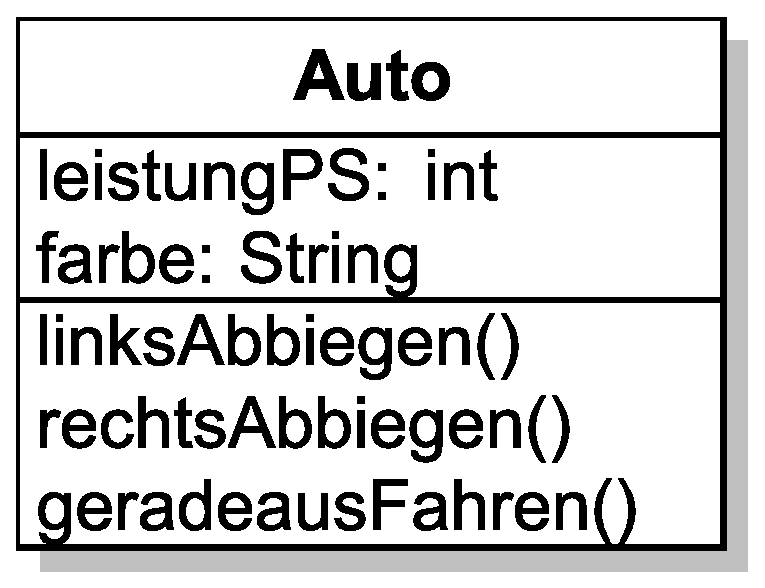
\includegraphics[width=0.2\textwidth]{./inf/SEKII/10_Java_Klassen/Auto.eps}
\end{center}

Das Diagramm einer Klasse ist in drei Abschnitte geteilt. In den obersten
Abschnitt wird der Name der Klasse geschrieben.

In den mittleren Abschnitt trägt man die Eigenschaften der Klasse ein, die für
das Programm, das generiert werden soll, von Bedeutung sind. Die Eigenschaften
bezeichnet man als Attribute. Wenn man die Klasse programmiert, wird für jedes
Attribut eine Variable angelegt. Der Datentyp der Variablen steht durch einen
Doppelpunkt getrennt hinter dem Namen des Attributs.

In den unteren Abschnitt schreibt man die Methoden, die auf die Objekte der
Klasse angewendet werden können.

In der Programmiersprache Java beschreibt eine Klasse das gemeinsame Schema für
alle ihre Objekte. Der Code wird nur einmal programmiert und automatisch auf
jedes Objekt angewendet, das zu der Klasse gehört.


\section{Beispiel: Klasse Hund}

\begin{minipage}{0.5\textwidth}
\begin{center}
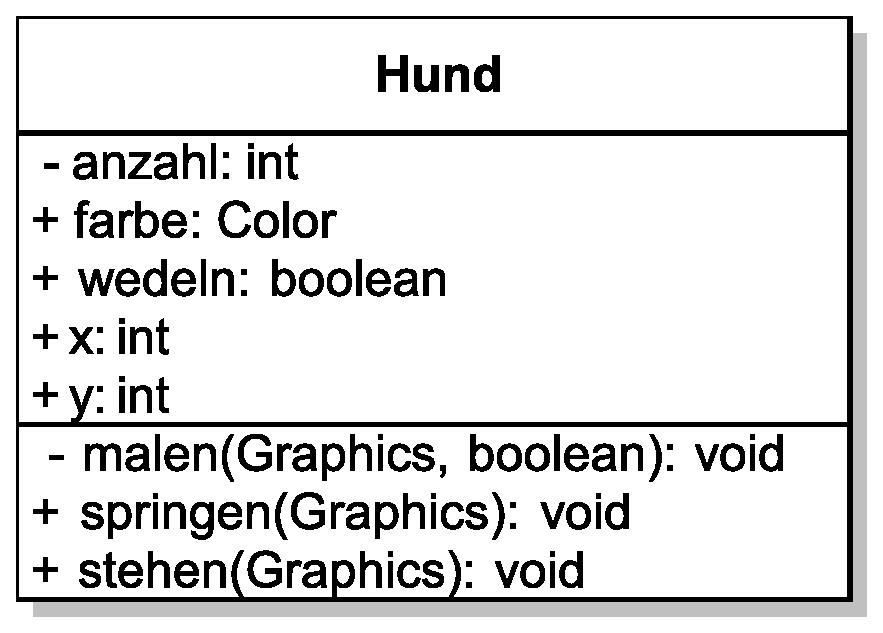
\includegraphics[width=0.66\textwidth]{./inf/SEKII/10_Java_Klassen/HundVorversion.eps}
\end{center}
\end{minipage}
\begin{minipage}{0.5\textwidth}
\subsubsection{Sichtbarkeit}

\lstinline|private| (-) : Variable/Methode kann
nicht von anderer Klasse aufgerufen
werden.

\lstinline|public| (+) : Variable/Methode kann
von jeder anderen Klasse aufgerufen
werden.
\end{minipage}

\subsection{Eine erste Version der Klasse Hund}

(Datei \myFile{HundVorversion.java} im Kurs-Repository)

\begin{lstlisting}
import java.awt.*;

public class Hund {
  public Color farbe = Color.LIGHT_GRAY;
  public boolean wedeln = false;
  public int x = 0;       æ// x- und y-Koordinate der
æ  public int y = 0;       æ// linken oberen Ecke
  // Klassenvariable: zählt die Anzahl aller Hunde - aber wann???
æ  static private int anzahl = 0;

  public void stehen(Graphics g) {     æ// malt den Hund stehend
æ    malen(g, true);
  }

  public void springen(Graphics g) {   æ// malt den Hund springend
æ    malen(g, false);
  }
  
  æ// "interne" Programmierung: malen() ist aus anderen Klassen heraus nicht sichtbar!
æ  private void malen(Graphics g, boolean stehen) {
    Color c = g.getColor();
    if (wedeln) {
      g.drawLine(x+0,y+0,x+10,y+20);
    } else {
      g.drawLine(x+0,y+40,x+10, y+20);
    }
    if (stehen) {
      g.drawLine(x+18, y+40, x+18, y+60);
      g.drawLine(x+20, y+40, x+20, y+60);
      g.drawLine(x+44, y+40, x+44, y+60);
      g.drawLine(x+46, y+40, x+46, y+60);
    } else {
      g.drawLine(x+18, y+40, x+0, y+52);
      g.drawLine(x+20, y+40, x+2, y+52);
      g.drawLine(x+44, y+40, x+56, y+52);
      g.drawLine(x+46, y+40, x+58, y+52);
    }
    g.setColor(farbe);
    g.fillRoundRect(x+10, y+15, 45, 25, 12, 12);
    g.fillOval(x+49,y+0,21,21);
    g.setColor(c);
    g.drawRoundRect(x+10, y+15, 45, 25, 12, 12);
    g.drawOval(x+49,y+0,21,21);
  }
}
\end{lstlisting}


\subsubsection{Was bedeutet static?}

Alle normalen (nicht \lstinline|static|) Variablen und Methoden beziehen sich
immer auf ein spezielles Objekt, dessen Namen man angeben muss.

\lstinline|static| Variable: Es gibt die Variable nur einmal pro Klasse.

\lstinline|static| Methode: Die Methode bezieht sich nicht auf ein einzelnes
Objekt und darf keine Objekt-Variablen verwenden.


Um Objekte der Klasse \myClass{Hund} in einem eigenen Programm zu nutzen würde
man jetzt wie folgt vorgehen. Zunächst würde man eine Variable vom Typ \myClass{Hund}
deklarieren:

\begin{lstlisting}
Hund felix;
\end{lstlisting}

Anschließend könnte man ein entsprechendes \myClass{Hund}-Objekt erzeugen:

\begin{lstlisting}
felix = new Hund();
\end{lstlisting}

Dazu wurde der sogenannte \emph{Konstruktor} der Klasse mit dem
\lstinline|new|-Operator aufgerufen. Ein Konstruktor hätte in der Klasse
\myClass{Hund} programmiert werden können. Aber in der ersten Version der Klasse
\myClass{Hund} ist davon nichts zu sehen.

Tatsächlich \emph{muss} man keinen Konstruktor programmieren. In diesem Fall
gibt es immer einen parameterlosen Konstruktor, der ein neues Objekt der Klasse
erzeugt. Dabei werden alle Objektvariablen so initialisiert, wie es in der
Klasse vorgegeben ist.

Das Hund-Objekt \lstinline|felix| hätte somit zu Beginn folgende Attributwerte:

\begin{tabular}{ll}
\lstinline|farbe| & \lstinline|Color.LIGHT_GRAY| \\
\lstinline|wedeln| \hspace{5mm} & \lstinline|false| \\
\lstinline|x| & \lstinline|0| \\
\lstinline|y| & \lstinline|0| \\
\end{tabular}

Da diese Attribute alle als \lstinline|public| deklariert wurden, lassen sich
diese Werte nun aus der Anwendungsklasse heraus problemlos ändern:

\begin{lstlisting}
felix.x = 100;
felix.y = 250;
felix.farbe = Color.BLACK;
felix.wedeln = true;
\end{lstlisting}

Um unser Hund-Objekt nun im Anwendungsprogramm auch sehen zu können, müssen wir
noch eine der beiden Methoden \lstinline|springen()| oder \lstinline|stehen()|
benutzen:

\begin{lstlisting}
felix.stehen(g);
\end{lstlisting}

Der \myClass{Graphics}-Kontext, den wir in \lstinline|myPaint()| automatisch
haben, ist der benötigte Parameter \lstinline|g|. Die Methoden zum Zeichnen der
Objekte werden also immer innerhalb von \lstinline|myPaint()| aufgerufen (bzw.
in Methoden, die ihrerseits in \lstinline|myPaint()| aufgerufen wurden und den
\myClass{Graphics}-Kontext als Parameter mit übernommen haben).

So weit so gut. Spätestens wenn du eine Hand voll Hunde erzeugt und mit
individuellen Attributwerten ausgestattet hast, wirst du dir jedoch eine
bequemere Methode zum Erzeugen von solchen Objekten wünschen. Wenn dir das nicht
sofort einleuchtet, dann solltest du es ausprobieren!


\subsection{Klasse Hund mit selbstdefinierten Konstruktoren}

Die Lösung besteht darin einen (oder auch mehrere!) Konstruktor in der Klasse
\myClass{Hund} zu programmieren (Datei \myFile{Hund.java} im Kurs-Repository).

Konstruktoren erkennst du daran, dass sie exakt den selben Namen wie die Klasse
tragen (und deshalb im Unterschied zu normalen Methoden auch mit einem
Großbuchstaben beginnen). Außerdem haben sie keinen Rückgabewert. Nicht einmal
das Schlüsselwort \lstinline|void|, welches normalerweise verwendet wird um bei
Methoden anzugeben, dass sie keinen Rückgabewert liefern, wird hier benutzt!

Wenn -- wie in unserem Beispiel hier -- mehrere Konstruktoren programmiert
werden, dann müssen sich diese anhand der Datentypen der Parameterliste
unterscheiden lassen. So kann es beispielsweise nicht zwei verschiedene
Konstruktoren in der selben Klasse geben, die beide als Parameter zwei Integer
Werte erwarten. Anhand der unterschiedlichen Parameterlisten kann der
Java-Compiler dann entscheiden, welcher der vorhandenen Konstruktoren im
konkreten Fall zu benutzen ist.

In unserer Klasse \myClass{Hund} werden vier Konstruktoren definiert. Wenn man
sich die Datentypen der Parameterlisten dieser vier Konstruktoren ansieht,
erkennt man, dass diese eindeutig voneinander unterscheidbar sind:

Liste der Konstruktoren der Klasse \myClass{Hund}:

\begin{tabular}{l}
\lstinline|Hund()| \\
\lstinline|Hund(int, int, Color)| \\
\lstinline|Hund(int, int, boolean)| \\
\lstinline|Hund(Color, boolean)| \\
\end{tabular}

\vspace{1mm}

\begin{lstlisting}
import java.awt.*;

public class Hund {
  public Color farbe = Color.LIGHT_GRAY;
  public boolean wedeln = false;
  public int x = 0;       æ// x- und y-Koordinate der
æ  public int y = 0;       æ// linken oberen Ecke
æ  static private int anzahl = 0; æ// Klassenvariable: Anzahl aller Hunde
æ
  public Hund() {
    wedeln = true;
    anzahl++;
  }

  public Hund(int xPos, int yPos, Color farbe) {
    x = xPos;
    y = yPos;
    this.farbe = farbe;
    wedeln = true;
    anzahl++;
  }

  public Hund(int x, int y, boolean wedeln) {
    this.x = x;
    this.y = y;
    farbe = Color.YELLOW;
    this.wedeln = wedeln;
    anzahl++;
  }

  public Hund(Color f, boolean w) {
    farbe = f;
    wedeln = w;
    anzahl++;
  }

  static public int getAnzahlHunde() {
    return anzahl;
  }

  public void stehen(Graphics g) {      æ// malt den Hund stehend
æ    malen (g, true);
  }
  
  public void springen (Graphics g) {   æ// malt den Hund springend
æ    malen (g, false);
  }

  private void malen (Graphics g, boolean stehen) {
    ...
  }
}
\end{lstlisting}


\section{Objekte erzeugen}

Eine Klasse gibt das Schema für eine Gruppe gleichartiger Objekte vor. Ein
konkret existierendes Objekt bezeichnet man auch als Instanz.

Zum Erzeugen eines Objektes (bzw. einer Instanz) einer Klasse muss man zunächst
eine Variable mit dem Typ der Klasse deklarieren, zum Beispiel:

\begin{lstlisting}
Hund hund1;
\end{lstlisting}

Schema:

\begin{lstlisting}
Klasse variablenname;
\end{lstlisting}

Diese Variable selbst enthält jedoch noch kein Objekt. Die Variable dient dazu
die Speicheradresse abzuspeichern, an der sich die Daten des Objektes im
Hauptspeicher befinden. Solange die Variable noch nicht auf ein Objekt zeigt,
hat sie den Wert \lstinline|null|. \lstinline|null| bedeutet „kein Objekt“.

Das Anlegen eines Objektes und das Abspeichern der Speicheradresse in der
Variablen geschieht zum Beispiel mit folgenden Befehlen:

\begin{lstlisting}
hund1 = new Hund();
hund2 = new Hund(50, 50, Color.YELLOW);
\end{lstlisting}

Schema:

\begin{lstlisting}
Variablename = new Klasse(Parameter);
\end{lstlisting}

Man kann die Deklaration und das Erzeugen des Objektes auch in einem Befehl
zusammen fassen:

\begin{lstlisting}
Hund hund1 = new Hund();
\end{lstlisting}

Wenn es für das Programm nützlich ist, kann man weitere Variablen auf dasselbe
Objekt zeigen lassen:

\begin{lstlisting}
Hund hilfe = hund1;   æ// hilfe zeigt auch auf hund1
\end{lstlisting}

Ein Objekt lebt solange, wie es Variablen gibt, die auf das Objekt verweisen.
Sobald es auf ein Objekt keinen Verweis mehr gibt, wird das Objekt vom System
automatisch vernichtet. Wenn man explizit sagen möchte, dass eine Variable auf
kein Objekt zugreift, so kann man ihr den Wert \lstinline|null| zuweisen:

\begin{lstlisting}
hund1 = null;
\end{lstlisting}


\section{Variablen einer Klasse}

Es gibt drei verschiedene Arten von Variablen, die in dem folgenden Beispiel
verdeutlicht werden:

\begin{lstlisting}
class Beispiel {
  static int klassenVariable;   æ// 1 mal pro Klasse
æ  int objektVariable;           æ// 1 mal pro Objekt
æ
  void methode() {
    int lokaleVariable;         æ// nur innerhalb von methode()
æ  }
}
\end{lstlisting}

\textbf{Klassenvariablen} beziehen sich auf alle Objekte der Klasse und sind
deshalb nur einmal vorhanden. Beispiel: Ein Zähler, der zählt, wie viele Objekte
der Klasse angelegt werden.

\textbf{Objektvariablen} speichern die Daten eines speziellen Objektes, z.B.\
die Farbe eines Hundes. Jedes Objekt besitzt seine eigenen Objektvariablen.

\textbf{Lokale Variablen} werden innerhalb einer Methode deklariert und werden
am Ende der Methode automatisch vom System wieder gelöscht.

Klassen- und Objektvariablen werden vom System automatisch mit \lstinline|0|
bzw.\ \lstinline|false| oder \lstinline|""| (leerer String) initialisiert.
Lokale Variablen dagegen haben zu Beginn einen unbestimmten Wert.


\subsection{Zugriff auf Variablen}

\begin{compactenum}[a)]
\item von außen

Von außen (d.h.\ von einer anderen Klasse aus) greift man auf Klassenvariablen
nach folgendem Schema zu:

\begin{lstlisting}
Klasse.attribut
\end{lstlisting}

Beispiel:

\begin{lstlisting}
Beispiel.klassenVariable = 10;
\end{lstlisting}

Auf eine Objektvariable kann man nur dann zugreifen, wenn man ein Objekt
besitzt. Schema:

\begin{lstlisting}
objekt.attribut
\end{lstlisting}

Beispiel:

\begin{lstlisting}
Beispiel bsp = new Beispiel();
bsp.objektVariable = 5;
\end{lstlisting}

\item innerhalb einer Klasse

Innerhalb einer Klasse kann man auf alle Klassen und Objektvariablen direkt
zugreifen ohne vorher den Klassen- oder Objektnamen anzugeben. Tatsächlich kann
man gar keinen „richtigen“ Objektnamen angeben, da die Klasse ja den Code für
alle Objekte darstellt. Um eine Objektvariable direkt anzusprechen (z.B. um sie
von einer lokalen Variablen mit dem gleichen Namen zu unterscheiden), kann man
das Objekt \lstinline|this| verwenden. \lstinline|this| bezeichnet das aktuelle
Objekt (analog zu dem menschlichen Ausdruck „ich“). In der Klasse Beispiel
könnte beispielsweise stehen:

\begin{lstlisting}
this.objektVariable = 10;
\end{lstlisting}
\end{compactenum}


\section{Methoden}

Methoden, die mit dem Schlüsselwort \lstinline|static| gekennzeichnet sind,
können jederzeit auch ohne Existenz eines Objektes aufgerufen werden. Sie
dürfen jedoch nur Klassenvariablen und lokale Variablen verwenden.

Alle nicht statischen Methoden, werden immer auf ein Objekt der Klasse
angewendet. Mit ihnen kann man die Objektvariablen des aktuellen Objektes
verändern.


\section{Konstruktor}

Der Konstruktor ist eine spezielle Methode, die vom System bei der Erzeugung
eines Objektes mit dem \lstinline|new| Operator aufgerufen wird. Er ist dazu
gedacht, Initialisierungen für das Objekt vorzunehmen (also Anfangswerte für
die Variablen des Objektes zu setzen). Das besondere:

\begin{compactitem}
\item Der Methodenname des Konstruktors ist mit dem Namen der Klasse identisch
\item Der Konstruktor besitzt keinen Rückgabewert (auch nicht
\lstinline|void|!). Aber er kann beliebig viele Parameter besitzen.
\item Der Konstruktor darf niemals explizit aus einer anderen Methode heraus
aufgerufen werden.
\end{compactitem}